%===============================================================
% Template using official colors of Czech Technical University.
% They are defined by new graphical manual - 2017.
% Specially designed for Laboratory of Structure of Biomolecules
% Share and modify as you like. Keep the name of the author.
% It is forbidden to use the template commercially.
% Author: Martin Malý.
% Published: 23.9.2017.
%===============================================================

\documentclass[aspectratio=169]{beamer}

\usepackage[utf8]{inputenc}
\usepackage{eqnarray,amsmath}
\usepackage{amsfonts}
\usepackage{amssymb}
\usepackage{graphicx}
\usepackage{lmodern} 
\usepackage{bm} 
\usepackage{epstopdf}
\usepackage{changepage}
\usepackage{array,booktabs}
\usepackage[most]{tcolorbox}
\usepackage{caption}
\usepackage{subcaption}
\usepackage{tikz}
\usetikzlibrary{positioning, arrows.meta, shapes, decorations.pathreplacing, calc}
\definecolor{ctublue}{HTML}{0000FF}
\definecolor{ctulightblue}{HTML}{ACD6EE}
\definecolor{ctuorange}{HTML}{F29830}
\colorlet{ctugray}{gray}
%\definecolor { ctublue } { cmyk } { 100, 43, 0, 0 }
%\definecolor { ctulightblue } { rgb }{ 172, 214, 238 }
%\definecolor { ctuorange } { hsb } { 22, 0.5, 1 }

\usetheme{default}
\setbeamercolor{section in toc}{fg=black,bg=white}
\setbeamercolor{alerted text}{fg=ctulightblue}
\setbeamercolor*{palette primary}{bg=ctublue,fg=gray!20!white}
\setbeamercolor*{palette secondary}{bg=ctulightblue,fg=white}
\setbeamercolor*{palette tertiary}{parent=palette primary}
\setbeamercolor*{palette quaternary}{fg=ctuorange,bg=gray!5!white}

\setbeamercolor*{sidebar}{fg=ctublue,bg=gray!15!white}


\setbeamercolor{titlelike}{parent=palette primary}
\setbeamercolor{frametitle}{parent=palette primary}

\setbeamercolor*{separation line}{}
\setbeamercolor*{fine separation line}{}

\setbeamertemplate{navigation symbols}{} 


\author{Vojtěch Klouda}
\title{Meta-prompty pro optimalizaci promptů velkého jazykového modelu}
\subtitle{Vedoucí práce: Ing. Jan Drchal Ph.D.}
\date[Event]{Obhajoba bakalářské práce\\18.6.2025}

\NewDocumentCommand{\hlbox}{m +m o}{%
  \begin{tcolorbox}[
    colback=#1!10!white,
    colframe=#1!80!black,
    boxrule=0.8pt,
    arc=4pt,
    left=6pt,
    right=6pt,
    top=4pt,
    bottom=4pt,
    enhanced,
    breakable,
    overlay={
      \IfValueT{#3}{%
        \node[anchor=north east, font=\scriptsize\bfseries, text=#1!80!black] 
        at (frame.north east) {#3};
      }
    }
  ]
  #2
  \end{tcolorbox}
}

%====================================================
%========== BEGINNING OF DOCUMENT ===================
%====================================================
\begin{document}

\begin{frame}
	\titlepage
	\begin{center}
  		
\includegraphics[height=1.3cm]{ctu_logo_black.pdf}
	\end{center}
\end{frame}


\logo{
\includegraphics[height=1cm]{ctu_logo_black.pdf}}



%\begin{frame}
%	\frametitle{Obsah} % představení, obsah  1 min
%	\begin{enumerate}
%		\item Motivace %  
%		\item Kontext % 
%		\item Metoda % 
%		\item Úlohy % 
%		\item Hlavní experiment %
%		\item Výsledky %
%		\item Shrnutí % 
%		\item Otázky oponenta % 
%	\end{enumerate}
%\end{frame}



\begin{frame}
	\frametitle{Motivace optimalizace promptů}
	\begin{itemize}
		%\pause
		\item Komplexní úlohy $\iff$ komplexní prompty
		\item Manuální ladění promptů vyžaduje čas a expertní znalosti
		\item Podobné prompty $\neq$ podobné účinky
		\item Data jsou potřeba i k manuálnímu ladění
		\item Méně náročné než fine-tuning
	\end{itemize}
\end{frame}		

% \begin{frame}
% 	\frametitle{Kontext}
% 	% Top half: two column
% {
% 	\setbeamercolor{itemize item}{fg=ctuorange}
% \begin{columns}[t] % align at top
%   \begin{column}{0.48\textwidth}
%     \hlbox{ctuorange}{
% 		\vspace{0.5em} 
% 		\begin{itemize}
% 			\item empiricky objevené škálovací zákony
% 			\item více dat, parametrů, epoch = lepší model
% 			\item zpomalující se růst
% 		\end{itemize}
% 	}[Training-time scaling]
%   \end{column}
%   \begin{column}{0.48\textwidth}
%     \hlbox{ctuorange}{
% 		\vspace{0.5em} 
% 		\begin{itemize}
% 			\item více výpočetního výkonu při volání
% 			\item Chain-of-thought
% 			\item myšlenkové struktury, agentické cykly
% 		\end{itemize}
% 	}[Inference-time scaling]
%   \end{column}
% \end{columns}
% }
% \vfill % push next content to bottom half (approx)
% %\pause
% % Bottom half: centered single column
% \begin{center}
%   \begin{minipage}{0.7\textwidth}
%     \centering
%     \hlbox{ctublue}{
% 		\vspace{0.5em} 
% 		\begin{itemize}
% 			\item přizpůsobení modelu na nějaký úkol
% 			\item fine-tuning, \textbf{optimalizace promptů}
% 		\end{itemize}
% 	}[Compile-time scaling]
%   \end{minipage}
% \end{center}

% \end{frame}

\begin{frame}
	\frametitle{Diagram použité metody}
	\begin{figure}[ht]
    \centering
	\scalebox{0.7}{
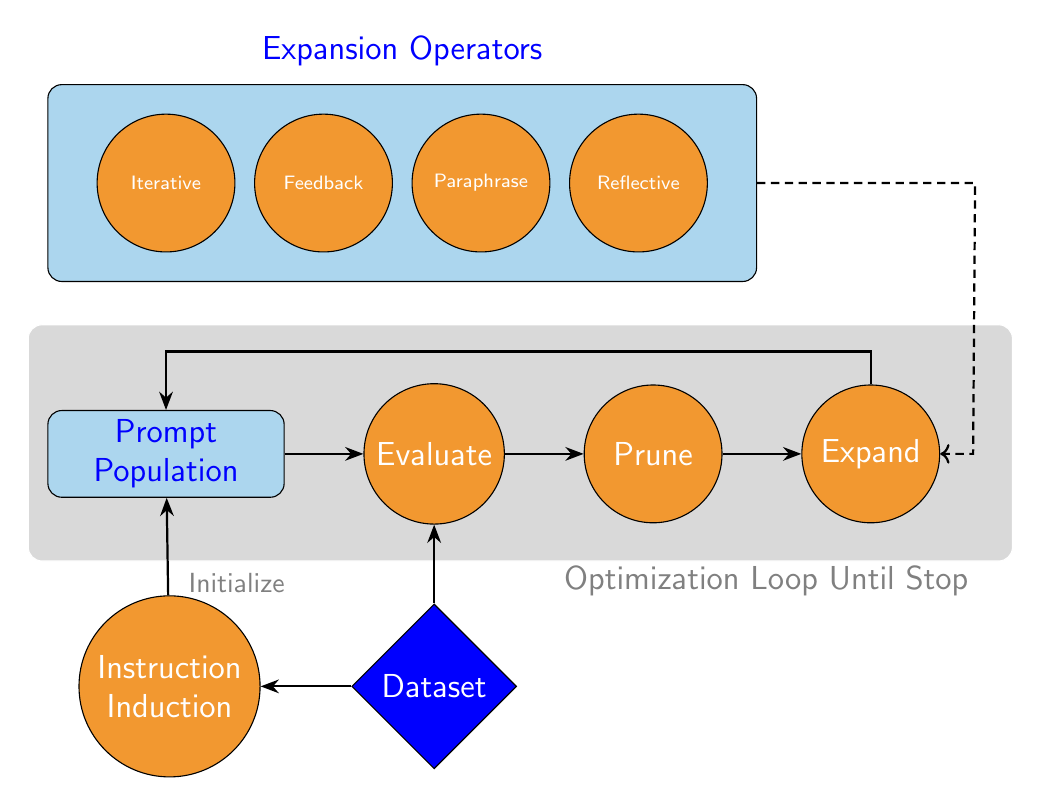
\begin{tikzpicture}[
    textnode/.style={
        draw, rectangle, rounded corners=5pt,
        fill=ctulightblue, text=ctublue,
        minimum width=3cm, minimum height=1cm, align=center
    },
    funcnode/.style={
        draw, circle, fill=ctuorange, text=white,
        minimum size=1.75cm, align=center
    },
    every node/.style={font=\sffamily\scriptsize},
    arrow/.style={-Stealth, thick},
    node distance=1cm and 1cm,
]

\node[textnode, minimum width=9cm, minimum height=2.5cm] (container) at (0,0) {};
\node[draw=white, rectangle,rounded corners = 5pt, minimum width=12.5cm, minimum height=3cm, fill=ctugray!30] (optimization) at (1.5,-3.3) {};
% Inner nodes positioned relative to container center
\node[funcnode] (iter) at ($ (container.center) + (-3cm,0cm) $) {Iterative};
\node[funcnode] (fb) at ($ (container.center) + (-1cm,0cm) $) {Feedback};
\node[funcnode] (para) at ($ (container.center) + (1cm,0cm) $) {Paraphrase};
\node[funcnode] (refl) at ($ (container.center) + (3cm,0cm) $) {Reflective};
\node[above=0.1cm of container, font=\large\sffamily, text=ctublue] {Expansion Operators};

\node[textnode, below=2cm of iter, font=\large\sffamily] (pop) {Prompt\\Population};

\node[funcnode, right=of pop, font=\large\sffamily] (eval) {Evaluate};
\node[funcnode, right=of eval, font=\large\sffamily] (prune) {Prune};
\node[draw, diamond, fill=ctublue, below=of eval, font=\large\sffamily, text=white] (data) {Dataset};
\node[funcnode, right=of prune, font=\large\sffamily] (expand) {Expand};
\node[funcnode, left=1.15cm of data, font=\large\sffamily] (init) {Instruction\\Induction};
\node[above right=0.5cm and 1cm of data, font=\large\sffamily, text=ctugray] {Optimization Loop Until Stop};
\node[above right =0.25cm and -0.7cm of init, font=\normalsize\sffamily, text=ctugray] {Initialize};

\draw[arrow] (data) -- (init);
\draw[arrow] (data) -- (eval);
\coordinate (rightcontainer) at ($(container)+(7.275,0)$);
\coordinate (rightexpand) at ($(expand)+(1.3,0)$);
\coordinate (aboveexpand) at ($(expand)+(0,1.3)$);
\coordinate (abovepop) at ($(pop)+(0,1.3)$);
\draw[->, thick, densely dashed] (container) -- (rightcontainer) -- (rightexpand) -- (expand);
\draw[arrow] (expand) -- (aboveexpand) -- (abovepop) -- (pop);
\draw[arrow] (init) -- (pop);
\draw[arrow] (pop) -- (eval);
\draw[arrow] (eval) -- (prune);
\draw[arrow] (prune) -- (expand);
\end{tikzpicture}
	}
    \caption{Diagram použité optimalizační metody}
    \label{fig:methoddiagram}
\end{figure}

\end{frame}

\begin{frame}
	\frametitle{Operátory pro generaci promptů}
	\hlbox{ctublue}{%\vspace{0.5em}
		\textbf{Data}: Příklady úloh z datasetu\\
		\textbf{Meta-prompt}: Najdi vhodnou instrukci pro řešení úlohy
	}[Instruction Induction]
	\hlbox{ctublue}{%\vspace{0.5em}
		\textbf{Data}: Prompty+skóre, vzestupně seřazené\\
		\textbf{Meta-prompt}: Vymysli prompt, který pokračuje v trendu
	}[Iterative]
	\hlbox{ctublue}{%\vspace{0.5em}
		\textbf{Data}: Špatný prompt a nevydařený pokus\\
		\textbf{Meta-prompt}: Odhal chybu a oprav prompt
	}[Reflective]
	\hlbox{ctublue}{%\vspace{0.5em}
		\textbf{Data}: Prompt \\
		\textbf{Meta-prompt}: Parafrázuj prompt
	}[Paraphrase]
\end{frame}

\begin{frame}
	\frametitle{Self-supervised optimalizace}
	\hlbox{ctublue}{%\vspace{0.5em}
		\textbf{Data}: Prompt a historie jeho porovnání s ostatními prompty pomocí LLM \\
		\textbf{Meta-prompt}: Najdi rozdíly mezi dobrými a špatnými prompty a udělej nový
	}[Feedback]
	{
		\setbeamercolor{itemize item}{fg=ctuorange}
		\hlbox{ctuorange}{%\vspace{0.5em}
			\textbf{Pro každý pár promptů:}
			\begin{itemize}
				\item Najdi úkoly, pro které oba prompty mají výsledky
				\item LLM porovná výsledky a prompty - vynese odůvodněný verdikt
				\item Verdikt se uloží do seznamu porovnání, využije ho Feedback operátor
			\end{itemize}
		}[Párová porovnávací metrika]

	}
\end{frame}

\begin{frame}
	\frametitle{Testovací úlohy}
	\hlbox{ctublue}{\vspace{0.5em}
		\begin{itemize}
			\item Kategorizace slov na základě netriviálních charakteristik
			\item Input: puff, domino, curl, placebo, ball, butterfly, halo, doodle
			\item Gold: ball, curl, doodle, puff; butterfly, domino, halo, placebo
		\end{itemize}
	}[Connections]
	\hlbox{ctublue}{\vspace{0.5em}
		\begin{itemize}
			\item Řešení úloh kompetetivního programování
		\end{itemize}
	}[CodeContests]
	\hlbox{ctublue}{\vspace{0.5em}
		\begin{itemize}
			\item Vlastní úloha - hledání dalšího čísla v posloupnosti
			\item Input: 0 3 22 9 44 15 66 21 88 27 110 33 132
			\item Output: 39
		\end{itemize}
	}[Posloupnosti]
\end{frame}

\begin{frame}
	\frametitle{Hlavní experiment}
	\begin{itemize}
		\item úlohy s objektivním řešením
		\item porovnání 4 operátorů
		\item 3 operátory používají metriky úloh
		\item 1 pracuje s porovnáváním výstupů pomocí LLM
		\item referenční řešení - rekonstrukce instrukcí z příkladů
		\item každý experiment zopakován třikrát
	\end{itemize}
\end{frame}

\begin{frame}
	\frametitle{Výsledky}
	\begin{figure}
		\includegraphics[width=8cm]{seq-table.pdf}
		\caption{Výsledky jednotlivých operátorů na úloze hledání dalšího čísla v celočíselné posloupnosti. Hard Baseline (HB) - nejlepší z 50 promptů z Instruction Induction operátoru, Soft Baseline (SB) - nejlepší z promptů inicializační populace.}
	\end{figure}
\end{frame}

\begin{frame}
	\frametitle{Výsledky}
	\begin{figure}
		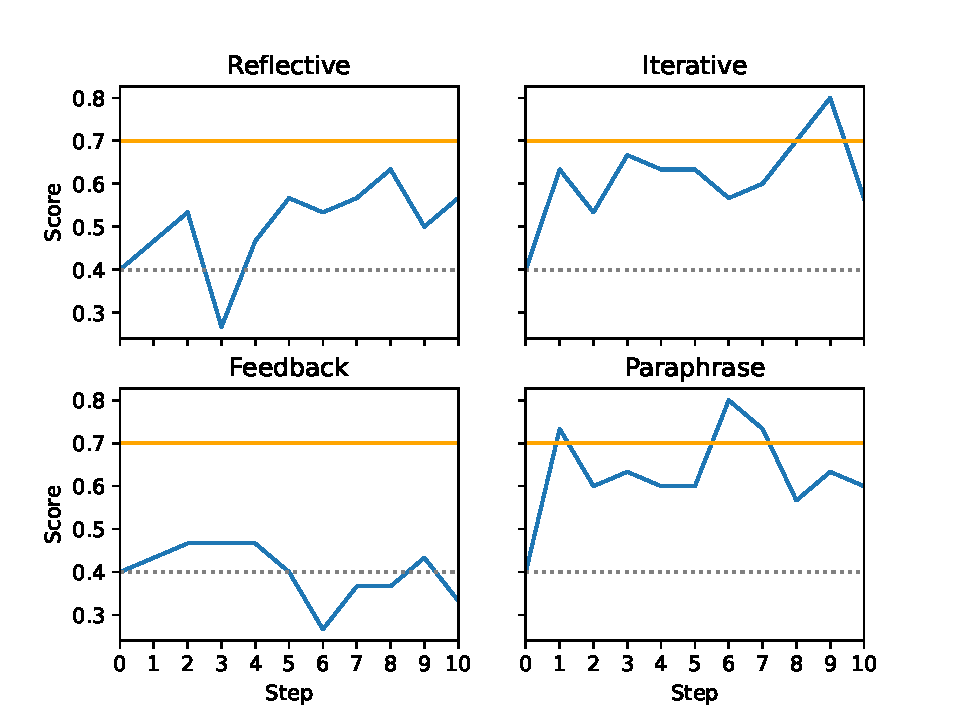
\includegraphics[width=8cm]{sequences.pdf}
		\caption{Výsledky jednotlivých operátorů na úloze hledání dalšího čísla v celočíselné posloupnosti. Hard Baseline (Oranžová) - nejlepší z 50 promptů z Instruction Induction operátoru, Soft Baseline (Šedá, čárkovaná) - nejlepší z promptů inicializační populace.}
	\end{figure}
\end{frame}

\begin{frame}
	\frametitle{Výsledky}
	\begin{figure}
		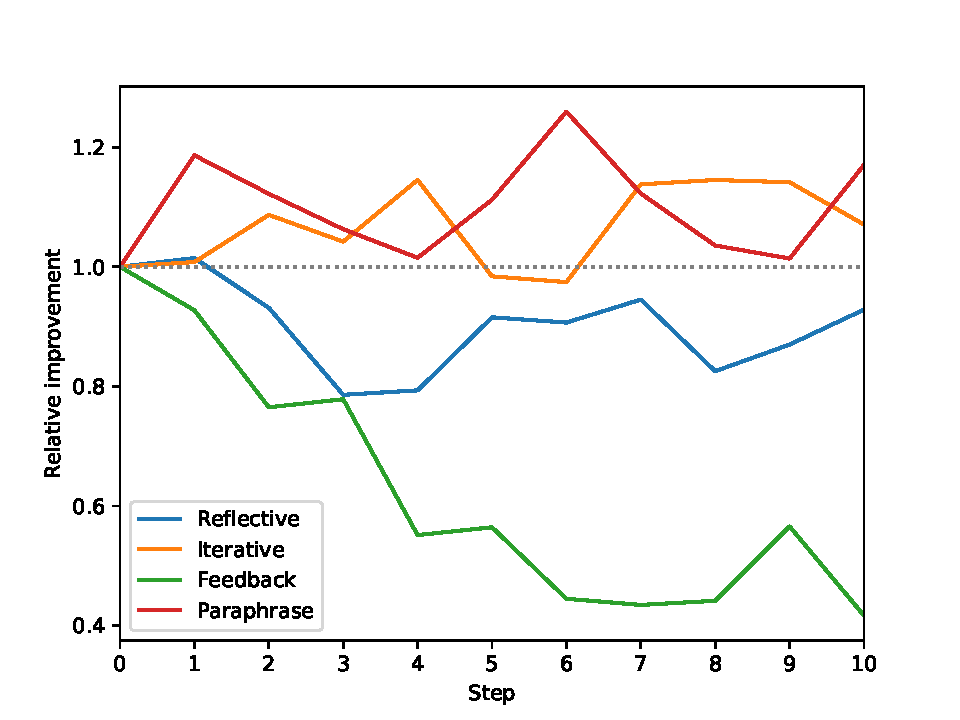
\includegraphics[width=8cm]{relative.pdf}
		\caption{Relativní zlepšení vzhledem k inicializačním promptům (Soft Baseline).}
	\end{figure}
\end{frame}

\begin{frame}
	\frametitle{Kreativní úlohy}
	\begin{figure}[htbp]
    \centering

    \begin{subfigure}{0.24\linewidth}
        \includegraphics[width=\linewidth]{image-gen0-id725f8.jpg}
        \caption{Initial}
    \end{subfigure}
    \hfill
    \begin{subfigure}{0.24\linewidth}
        \includegraphics[width=\linewidth]{image-gen1-id534fc.jpg}
        \caption{Step 1}
    \end{subfigure}
    \hfill
    \begin{subfigure}{0.24\linewidth}
        \includegraphics[width=\linewidth]{image-gen2-id62971.jpg}
        \caption{Step 2}
    \end{subfigure}
    \hfill
    \begin{subfigure}{0.24\linewidth}
        \includegraphics[width=\linewidth]{image-gen3-id4cf7b.jpg}
        \caption{Step 3}
    \end{subfigure}

    \caption{Využití operátoru Feedback pro kreativní úlohu - generace promptu pro difuzní obrázový model pro daná přídavná jména: ``wistful'', ``hopeful'' and ``lonely''.}
    \label{fig:wistful}
\end{figure}
\end{frame}

\begin{frame}
	\frametitle{Shrnutí}
	\begin{itemize}
		%\pause
		\item rozsáhlý přehled literatury
		%\pause
		\item zasazení do kontextu jiných metod škálování
		%\pause
		\item modulární optimalizační metoda promptů
		\item 5 operátorů včetně self-supervised operátoru Feedback
		%\pause
		\item framework pro strukturovanou generaci s inference-time metodami
		%\pause
		\item porovnání operátorů na různých úlohách oproti silnému referenčnímu řešení
	\end{itemize}
\end{frame}

\begin{frame}
	\frametitle{Otázky oponenta}
	\hlbox{ctuorange}{\vspace{0.5em}Do jaké míry lze navržené řešení použít obecně v praxi, např. pro úlohu převodu PDF obsahu na strukturovaný
JSON výstup?}[Otázka]

	\hlbox{ctublue}{\vspace{0.5em}
		\begin{itemize}
			\item Prompt lze optimalizovat pro jakoukoliv úlohu, kde je dobře definovaná metrika a jsou dostupná data, případně lze použít LLM v hodnotící roli. 
			\item Čím komplexnější úkol, tím složitějsí a delší prompt a tím větší hledací prostor. 
			\item Vedoucí práce používá optimalizaci promptům v úlohách NLP, jako například rozpoznávání entit v novinových článcích.
		\end{itemize}
	}[Odpověď]
	
\end{frame}

\begin{frame}
	\frametitle{Otázky oponenta}

	
\hlbox{ctuorange}{\vspace{0.5em}Jakým způsobem je zajištěno, že párové hodnocení promptů a jejich výsledků nevede ke zhroucení
prohledávání pouze na úzkou oblast prostoru? Jsou nějaké zkušenosti s nasazením v obecných praktických
úlohách?}[Otázka]

	\hlbox{ctublue}{\vspace{0.5em}
		\begin{itemize}
			\item Problém diverzity byl velkým tématem pro všechny operátory, nejen pro operátor Feedback, který staví na párovém porovnávání.
			\item Každé volání operátoru Feedback používá náhodně vybraný prompt, jehož historie porovnáváním je pak využita ke generaci nového promptu.
		\end{itemize}
	}[Odpověď]
\end{frame}

\begin{frame}
	\frametitle{Otázky oponenta}

	\hlbox{ctublue}{\vspace{0.5em}
		\begin{itemize}
			\item Operátor Feedback měl suveréně nejhorší výsledky a docházelo ke kolapsu vyhledávání.
			\item Nejdůležitější mi přijde diverzita u inicializační populace a u Instruction Induction přidávám seed v podobě Persony.
			\item Obecně jsem se tento problém snažil řešit prořezáváním duplikátů v populaci na základě editační vzdálenosti a dále v rámci návrhu meta-promptů.
			\item Článek, kterým jsem se při návrhu metody inspiroval, ji testuje například na MT-Bench, což je soubor úkolů, testující užitečnost odpovědí LLM při vícekrokových konverzacích. Často se také k testování používají například reálná řešení z Githubu.
		\end{itemize}
	}[Odpověď]
\end{frame}

\begin{frame}
	\begin{center}
		\Large{Děkuji za pozornost}
	\end{center}
\end{frame}
\end{document}
